\chapter{Background and Related Work}
\label{cha:background}

A large part of the work undertaken during this project requires a significant understanding on how a particular deep learning architecture, the Transformer works. In this section, we will cover some of the required background and insights drawn from the Transformer architecture which were needed to model and solve our problem of prediction on packet data. We also present adaptations of the Transformer architecture to solve problems in several fields such as NLP/CV and relevant ideas which could be adapted to our tasks.

\section{Background on Transformers}
\label{sec:background}

\subsection{Sequence modelling with attention}
\label{ssec:bgsequence}

Transformers are built around the \emph{attention mechanism}, which maps an input sequence to an output sequence of the same length.
Every output encodes its own information and its context, ie information from related elements in the sequence, regardless of how far they are apart.
The process involves the scalar multiplication of the input feature matrix attention matrix as a dot product operation, which allows the deep neural network to focus on certain parts of the sequence at a time, based on the values of the attention weight matrix. This allows the network to attend to parts of the sequence in parallel, rather than in sequence, which allows highly efficient computation. Also, as the attention weights are learnable parameters for the network, the Transformer over time, learns to choose the best weights which allow optimum learning of structure within the sequence of data.
Computing attention is efficient as all elements in the sequence can be processed in parallel with matrix operations that are highly optimised on most hardware. These properties have made Transformer based neural networks the state-of-the-art solution for solving many sequence modelling tasks. We refer to an excellent illustrated guide to the Transformer here\cite{trans}.


While attention originated as an improvement to Recurrent Neural Networks(RNNs), it was soon realised that the mechanism could replace them entirely.\cite{vaswaniAttentionAllYou2017}
RNNs were the initial state-of-the art deep learning architectures in sequence modelling problems, however they suffer from several issues. Training RNNs is usually limited by one or all of the following problems:
\begin{enumerate}
\item RNNs are not computationally efficient for training long sequences, as they require $n$ sequential operations to learn a sequence, $n$ being the length of the given sequence. This makes the training process extremely slow.
\item RNNs suffer from the problem of \emph{vanishing gradients} \ie as elements in the input need to be processed in a sequence over time, the gradients used by the optimiser\cite{Robbins2007ASA} for the elements at the end of very long sequences, become extremely small and numerically unstable to converge to the desired value.
\item RNNs struggle to learn \emph{long-term dependencies}, \ie learning relations between elements far apart in the sequence is challenging.
\end{enumerate}

We present an excellent summary of the challenges and differences between several deep learning architectures which have attempted to solve the sequence modelling problem in Table \ref{bg:table1}.

\begin{table}[htbp]
\centering
\begin{tabular}{ c   c   c  c  }
\toprule
Layer Type & Complexity   & Sequential   & Maximum \\
& per Layer & Operations & Path Length \\
\midrule
Transformer(Self-Attention) & $O(n^2 \cdot d)$ & $O(1)$ & $O(1)$ \\
Recurrent NN & $O(n \cdot d^2)$ & $O(n)$ & $O(n)$ \\
Convolutional NN & $O(k \cdot n \cdot d^2)$ & $O(1)$ & $O(\log_{k}{n})$\\
Restricted(Self-Attention) & $O(r \cdot n \cdot d)$ & $O(1)$ & $O(n/r)$\\
\bottomrule
\end{tabular}
\caption{Maximum path lengths, per-layer complexity and minimum number of sequential operations
for different layer types. $n$ is the sequence length, $d$ is the representation dimension, $k$ is the kernel
size of convolutions and $r$ the size of the neighbourhood in restricted self-attention.
SOURCE: Original paper\cite{vaswaniAttentionAllYou2017}}
\label{bg:table1}
\end{table}


Augmenting RNNs with attention solves some of these issues\cite{rnnattention},  and replacing them with \emph{Transfomers} has shown to solve all these problems.
The authors propose an architecture for translation tasks that contains:
\begin{itemize}
\item a learnable \emph{embedding} layer mapping words to vectors
\item a \emph{transformer encoder} encoding the input sequence
\item a \emph{transformer decoder} generating an output sequence based on the encoded input
\end{itemize}

Each transformer block alternates between attention and linear layers, ie between encoding context and refining features. The attention mechanism helps learn "context rich" representations of every element, mapping relevant information from the surrounding elements which surround it and the linear layers help map this learn information into a form useful for downstream prediction. Figure \ref{fig:transformer} shows details of the original Transformer architecture and the functions of its layers.

\begin{figure}[!hbt]
  \begin{center}
    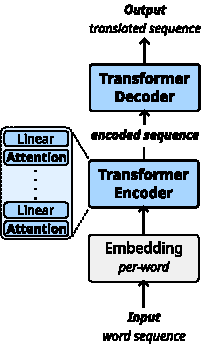
\includegraphics[scale=1.5]{figures/architecture_transformer.pdf}
    \caption{Original Transformer Architecture, Credits: Alex, HotNets '22}
    \label{fig:transformer}
  \end{center}
\end{figure}

\subsection{Pre-training and fine-tuning}
\label{ssec:bgtraining}

Due to the highly efficient and parallelizable nature of Transformers, they can be widely used a variety of tasks based on the principle of \emph{transfer learning}. The most common strategy for that is to use the architecture for two phases, \emph{pre-training} and \emph{fine-tuning}. Inspired by the original Transformers success on the task of language translation, the use of Transformers has become ubiquitous in solving NLP problems. We present one such state of the the art NLP Transformer model, 
called BERT\cite{devlinBERTPretrainingDeep2019}, one of the most widely used transformer models today.
While the original Transformer had both an encoder and decoder with attention, BERT uses only the transformer encoder followed by a small and replaceable decoder. This decoder is usually a set of linear layers and acts as a multilayer perceptron (MLP); and is usually called the 'MLP head' in the deep learning community. The principle of transfer-learning works for BERT as follows:

\begin{itemize}
\item In the first step, BERT is \emph{pre-trained} with a task that requires learning the underlying language structure. Linguists' research has shown that a Masked Language Model is optimal for deep learning models for learning structure in natural languages.\cite{wettigShouldYouMask}
Concretely, a fraction of words in the input sequence is masked out (15\% in the original model), and the decoder is tasked to predict the original words from the encoded input sequence.
BERT is used to generate contextual encodings of, which is only possible due to the bi-directionality of the attention mechanism in BERT. This allows the model to infer the context of the word from both sides in a given sentence, which was not possible earlier when elements in a sequence were only processed in a given order.\footnote{
    BERT is pre-trained from text corpora with several billion words and fine-tuned with $\sim$100 thousand examples per task.
}

\item In the second step, the unique pre-trained model can be fine-tuned to many different tasks by replacing the small decoder with task-specific ones, eg language understanding, question answering, or text generation.
The fine-tuning process involves resumption of learning from the saved weights of the pre-training phase, but for a new task or learning in a new environment. The new model has already learned to encode a general language context and only needs to learn to extract the task-relevant information from this context.This requires far less data compared to starting from scratch and makes the pre-training process faster.

Furthermore, BERTs pre-training step is unsupervised/self-supervised, \ie it requires only ``cheap'' unlabelled data and no labelled signal from the data a target value. As procuring labelled data is harder, this problem is mitigated by having a pre-training phase on ``generic" data and then using 
``expensive'' labeled data, eg for text classification, during the fine-tuning phase. Figure \ref{fig:bert} shows the details of BERT's pre-training and fine-tuning phase.
\end{itemize}

\begin{figure}[!hbt]
  \begin{center}
    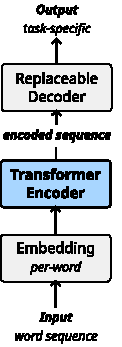
\includegraphics[scale=1.5]{figures/architecture_bert.pdf}
    \caption{Original BERT Architecture, Credits: Alex, HotNets '22}
    \label{fig:bert}
  \end{center}
\end{figure}



Another extremely useful feature of Transformer is its generalization ability, which is  possible due to its highly efficient parallelization during training, which in turn helps transfer of knowledge to a variety of tasks during the process of fine-tuning. The OpenAI GPT-3\cite{brownLanguageModelsAre2020} model that investigates few-shot learning with only a pre-trained model.
As it is just a pre-trained model, it does not outperform fine-tuned models on specific tasks. However, GPT-3 delivers impressive performance on various tasks, including translation, determining the sentiment of tweets, or generating completely novel text. As per requirement, it can also be fine-tuned on specific tasks, which showcases further, the generalization power of transformers.


\subsection{Vision transformers}
\label{ssec:bgvit}

Following their success in NLP, the use of Transformers were explored as a possibility to learn structural information in other kinds of data. One such field where they gained a lot of traction in in the field of CV.
However adapting the use of Transformers to vision tasks came with a few major challenges: 
\begin{itemize}
\item Image data does not have a natural sequence, as they are a spatial collection of pixels.
\item Learning encodings at the pixel level for a large number of images, proved to be too fine-grained to scale to big datasets.
\item The Masked Language Model theory couldn't be efficiently transferred to the context of learning structure in images, as the relationship between the units (pixels) does not follow the same logic as in natural languages.
\end{itemize}

To solve this problems, the authors of the Vision Transformer(ViT)\cite{dosovitskiyImageWorth16x162021}, came up with multiple ideas to solve each of these problems, in order to have the data in a form, on which a Transformer could be efficiently trained.
\begin{itemize}
\item \emph{Serialize and aggregate the data: } As image data does not have a natural sequence structure, such a structure was artificially introduced. Every image was split at the pixel level and aggregated into patches of dimension 16$\times$16 and each of these patches became a member of the new input ``sequence". As Transformers scale quadratically with increasing sequence size \ref{bg:table1}, this also solved the problem of efficiency and that encodings at the pixel level are too fine-grained to be useful. The embedding and transformer layers were then applied to the resulting sequence of patches, using an architecture similar to BERT.
\item \emph{Domain Specific Pre-training: } At the heart, most CV problems have very similar training and inference objectives, one of the most common being image classification, which makes most of the vision tasks similar in objective, differing only in environment. This made classification a much more suited task for image data pre-training as opposed to masking and reconstruction. This was exploited by the ViT and both the pre-training and fine-tuning was done with the objective of classification, with only a change in environment between the stages. This also meant that understanding structure in image data, not only required information from the neighbouring patches but also from the whole image, which was possible by using all the encoded patches for classification. We present the details of ViT's pre-training and fine-tuning in Figure \ref{fig:vit}
\end{itemize}

\begin{figure}[!hbt]
  \begin{center}
    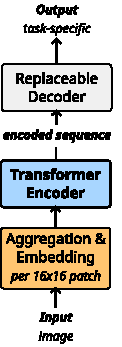
\includegraphics[scale=1.5]{figures/architecture_vit.pdf}
    \caption{Original ViT Architecture, Credits: Alex, HotNets '22}
    \label{fig:vit}
  \end{center}
\end{figure}


Finally, ViT's authors also observe that domain-specific architectures that implicitly encode structure, like convolutional networks (CNNs) work extremely well for image datasets and  actually result in better performance on small datasets.However, given enough pre-training data, learning sequences with attention beats architectures that encode structure implicitly, making the process a tradeoff between the utility and the amount of resources required for pre-training. Later research in the field has also shown advancements in vision based transformers which use a masked reconstruction approach\cite{heMaskedAutoencodersAre2021}, such details however are beyond the scope of this section. 


\section{Related Work}
\label{sec:related_work}

Direct comparison wise, there is not much to add here. We claim that no one really tried to solve this problem as it was a ``lost" cause. However, we will add some ML in Networking examples as, as we did look at them to an extent. For the relevant ML part, the previous section covers Transformers in more than enough detail.

Will mention a bit about 
\begin{itemize}
\item MimicNet\cite{zhangMimicNetFastPerformance2021}
\item Puffer\cite{puffer} 
\item Aurora\cite{jayDeepReinforcementLearning2019}
\item Pensieve\cite{maoNeuralAdaptiveVideo2017}
\item More can be added later  
\end{itemize}



